\subsection{SPMD at Nano-Scale}
\label{sec:modelling_nano}

%% 1. Introduction: How to get more variations
%% 2. How to generate the equations
%% 3. Explain Alignment how power monitor is aligned with event trace
%%    3a. Explain gradient method to align 
%% 4. Explain the results
%%    4a. Explain problems in CPU Base power
%%    4b. Explain problems in per-core CPU power
%%    4c. Explain problems in GPU
%% 5. Reasons for the equation not giving correct solution
%% 6. Conclusion

Given that the {\color{blue}CPU/GPU utilization level variation} seems to mainly exist within
each rendering interval yet creating two equations per interval is
not enough, we next explore setting up multiple equations, each
at an even finer scale, within each 16.7ms interval. We denote this
approach as {\it SPMD at nano-scale}.

\paragraph{Methodology.}
The methodology is similar to that of micro-scale SPMD, except that
instead of generating two equation per 16.7 ms interval, we generate
16 equations, \ie one equation for every 1ms sub-interval.  We tried
to set up one system for 1, 2, 4, and 8 16.7ms intervals and show results for 1
interval, \ie 16 equations.  The other results are
very similar and are omitted due to page limit.
\begin{figure*}[tp]
    \centering
     \begin{subfigure}[b]{\textwidth}
         \centering
         
\includegraphics[width=\textwidth]{figures/label_macro_equations.png}
    \end{subfigure}
    \\
    \centering
     \begin{subfigure}[b]{0.32\textwidth}
         \centering
         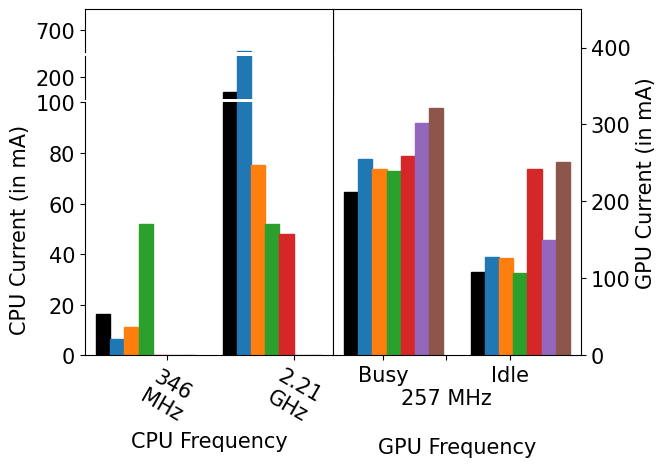
\includegraphics[width=\textwidth]{figures/002_Pixel2_1_nano_equations.png}
         \label{fig:nano_equations_p2}
         \vspace{-0.25in}
         \caption{Pixel 2: TPMD vs nano-SPMD coefficients}
     \end{subfigure}
    \begin{subfigure}[b]{0.32\textwidth}
         \centering
         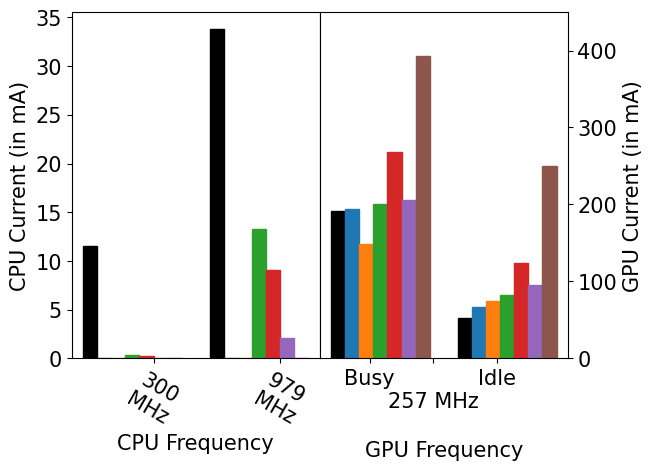
\includegraphics[width=\textwidth]{figures/003_MotoZ3_1_nano_equations.png}
         \label{fig:nano_equations_z3}
         \vspace{-0.25in}
         \caption{Moto Z3: TPMD vs nano-SPMD coefficients}
     \end{subfigure}
    \begin{subfigure}[b]{0.32\textwidth}
         \centering
         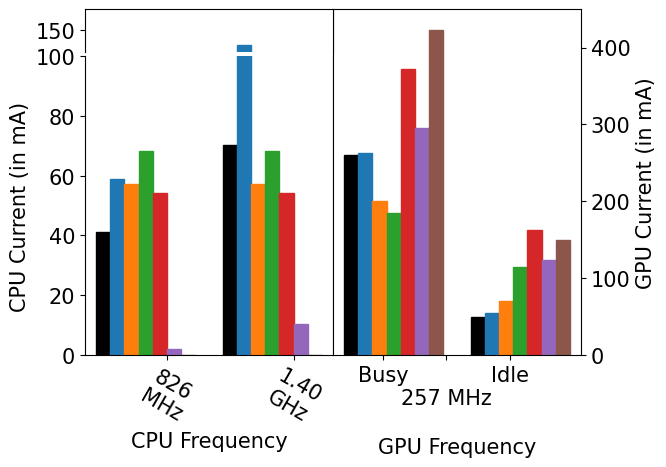
\includegraphics[width=\textwidth]{figures/004_Pixel4_1_nano_equations.png}
         \label{fig:nano_equations_p4}
         \vspace{-0.25in}
         \caption{Pixel 4: TPMD vs nano-SPMD coefficients}
     \end{subfigure}
     \hfill
     \vspace{+0.1in}
     \centering
     \begin{subfigure}[b]{0.31\textwidth}
        \centering
	    \caption{Pixel 2: TPMD vs nano-SPMD error}
	    \vspace{-0.05in}
    	{ \scriptsize
%    	\begin{tabular}{ | p{1.3cm} | p{.2cm} | p{.2cm} | p{.2cm} | p{.2cm} | p{.2cm} | p{.2cm} | }
        \begin{tabular}{ | p{1.8cm} | p{.2cm} | p{.2cm} | p{.2cm} | p{.2cm} | p{.2cm} | p{.2cm} | }
%    	\begin{tabular}{ | l | c | c | c | c | c | c | }
    		\hline
    		     & \multicolumn{6}{ c|}{Error for each App Sc. (\%)}\\
    		\cline{2-7}
                    Model & \rot{B. Menu} & \rot{B. Still} & \rot{C. Menu} & \rot{C. Still} & \rot{M. Menu} & \rot{M. Still}  \\
    		\hline
                Fix. F. Const.       & 4.3 & 3.8 & 12 & 9.1 & 13 & 16 \\
                TPMD                 & 19 & 30 & 23 & 22 & 22 & 31 \\
    		\hline
    	\end{tabular}
    	}
    	% \vspace{-0.05in}
	    % \caption{Pixel 2: TPMD vs nano-SPMD error}
    \end{subfigure}
    \hfill
    \begin{subfigure}[b]{0.31\textwidth}
        \centering
	    \caption{Moto Z3: TPMD vs nano-SPMD error}
	    \vspace{-0.05in}
    	{ \scriptsize
%    	\begin{tabular}{ | p{1.3cm} | p{.2cm} | p{.2cm} | p{.2cm} | p{.2cm} | p{.2cm} | p{.2cm} | }
        \begin{tabular}{ | p{1.8cm} | p{.2cm} | p{.2cm} | p{.2cm} | p{.2cm} | p{.2cm} | p{.2cm} | }
%    	\begin{tabular}{ | l | c | c | c | c | c | c | }
    		\hline
    		     & \multicolumn{6}{ c|}{Error for each App Sc. (\%)}\\
    		\cline{2-7}
                    Model & \rot{B. Menu} & \rot{B. Still} & \rot{C. Menu} & \rot{C. Still} & \rot{M. Menu} & \rot{M. Still}  \\
    		\hline
                Fix. F. Const.       & 14 & 14 & 7.3 & 14 & 21 & 7.8 \\
                TPMD                 & 42 & 18 & 39 & 27 & 41 & 41 \\
    		\hline
    	\end{tabular}
    	}
    	% \vspace{-0.05in}
	    % \caption{Moto Z3: TPMD vs nano-SPMD error}
    \end{subfigure}
    \hfill
    \begin{subfigure}[b]{0.31\textwidth}
        \centering
    	\caption{Pixel 4: TPMD vs nano-SPMD error}
    	\vspace{-0.05in}
    	{ \scriptsize
%    	\begin{tabular}{ | p{1.3cm} | p{.2cm} | p{.2cm} | p{.2cm} | p{.2cm} | p{.2cm} | p{.2cm} | }
        \begin{tabular}{ | p{1.8cm} | p{.2cm} | p{.2cm} | p{.2cm} | p{.2cm} | p{.2cm} | p{.2cm} | }
%    	\begin{tabular}{ | l | c | c | c | c | c | c | }
    		\hline
    		     & \multicolumn{6}{ c|}{Error for each App Sc. (\%)}\\
    		\cline{2-7}
                    Model & \rot{B. Menu} & \rot{B. Still} & \rot{C. Menu} & \rot{C. Still} & \rot{M. Menu} & \rot{M. Still}  \\
    		\hline
                Fix. F. Const.       & 13 & 11 & 16 & 27 & 21 & 26 \\
                TPMD                 & 38 & 50 & 23 & 42 & 29 & 34 \\
    		\hline
    	\end{tabular}
    	}
    	% \vspace{-0.05in}
    	% \caption{Pixel 4: TPMD vs nano-SPMD error}
    \end{subfigure}
    \hfill
    \caption{Model parameters derived by nano-scale SPMD. (Showing the top 2 CPU
        frequencies with high CPU utilization.)(The GPU parameter for the TPMD
        is represented by average over all app scenarios GPU parameters.) }
    \vspace{-0.1in}
    \label{fig:nano_equations}
\end{figure*}

\paragraph{Results.}
Figure~\ref{fig:nano_equations} shows the model parameters output of the 
Fix. F. Const. regression solver for the same 6 app scenarios.  We
observe that the model parameters derived from nano-scale SPMD are
also drastically different from the corresponding parameters derived
from the TPMD model.  In particular, 
(1) the power models output
by the solver have high LSF error,
between (3.75\%-16.40\%) for Pixel 2,
between (7.29\%-20.61\%) for Moto Z3,
and between (11.28\%-26.58\%) for Pixel 4;
% (2) For Pixel 4, out of the 6 app scenarios, the CPU parameters are zero for 2
%  scenarios and less than 50\% of the TPMD counterparts for 3
%  scenarios.  Similarly, the CPU parameters are zero for 2 scenarios and
%  less than 50\% of thei TPMD counterprts for 4 scenarios for
%  Moto Z3.  Finally, the CPU parameters are zero \comment{for all scenarios???} for Pixel 2.
(2) the power parameters are
0.0$\times$-2.76$\times$,
0.0$\times$-0.57$\times$,
0.0$\times$-1.62$\times$ of their
counterparts for CPU frequency respectively for the 3 phones; and
(3) the individual power parameters are
1.02$\times$-1.48$\times$,
0.78$\times$-1.92$\times$,
0.50$\times$-1.43$\times$ of their
counterparts for GPU Busy frequency and
0.72$\times$-2.08$\times$,
0.74$\times$-8.60$\times$,
1.09$\times$-21.60$\times$ of their
counterparts for GPU Idle frequency in the TPMD model for Pixel 2,
Moto Z3, and Pixel 4, respectively.
 
 \comment{so,do we reject these results? on what basis? need to echo section 3.4}
 
{\color{blue}We report the corresponding  $R^2$-measurement and F-test in Table~\ref{tab:nano_rank_singular}.--EXPLAIN THOSE VALUES-- Still SMPD does not give a reasonable valid modeling results.}
\dcomment{
We observe that the $R^2$ varies between 0.25-0.96, 0.34-0.95 and 0.63-0.93 for the
three phones respectively. Similar to micro, we observe that for some app scenarios the
curve\_fit fail \eg for Candy Crush Still on Pixel 4 has the lowest 
$R^2$ value of 0.63. It's has the highest average error of 27\%.
and having the minimum singular value was 0.39. 
Here the system's susceptibility to noise can be
estimated to be $0.39^{-1} \approx 2.6\times$ the measurement noise.
% From $\|\epsilon_m\|_2/\min\text{eig}(\mathbf{X})$, explained in
% \S\ref{subsec:contri} NEED TO CONCLUDE.
The the minimum singular values are between
0.20-0.77,
0.50-0.91
and
0.29-1.07 for the 3 phones respectively.
} 
 
\begin{table}[tb]
{\footnotesize
    \centering
    \caption{The 2 smallest singular values for the set of equations for nano-scale "Fix-Freq.-Constr. SPMD" for Pixel 4  for 16 equation system of equation.
    (Top 4 singular values are shown.)
    }
    \vspace{-0.1in}
    % \begin{tabular}{|c|p{9mm}|p{4.5mm}|p{4.5mm}|p{4mm}|p{4mm}|p{4mm}|c|}
    % \hline
    %     App & Scenario & Num. of Eqns. & Num. of Vars. &  \multicolumn{3}{c|}{Smallest Singular Values} & $R^{2}$ \\
    \begin{tabular}{|c|p{10.5mm}|p{7.5mm}|p{7.5mm}|c|c|c|}
    \hline
        App & Scenario & Num. & Num. &  \multicolumn{2}{c|}{Singular}  & $R^{2}$ \\
            &          &  of &   of &  \multicolumn{2}{c|}{Values}  &   \\
            &          & Eqns. & Vars. &  \multicolumn{2}{c|}{}  & \\
        \hline
        \multirow{2}{13mm}{Bricks Breaker} & Menu & 16 & 4  & 1.42  & 1.07 & 0.93 \\
         \cline{2-7}
         & Still & 16 & 4 & 1.31  & 1.01 & 0.87 \\
         \hline
        \multirow{2}{13mm}{Candy Crush S.} & Menu & 16 & 4  & 1.25 & 0.29 & 0.81 \\
        \cline{2-7}
	     & Still & 16 & 4 & 0.87  & 0.39 & 0.63 \\
	     \hline
         \multirow{2}{13mm}{Mini Golf 3D} & Menu & 16 & 5 & 1.68  & 0.51 & 0.73 \\
         \cline{2-7}
         & Still & 16 & 5 & 0.75 & 0.48 & 0.77 \\
         \hline
    \end{tabular}
    \label{tab:nano_rank_singular}
    \vspace{-0.1in}
}
\end{table}

\begin{table}[tb]
    \centering
    \caption{Equations for the 16.7 ms interval for Bricks Breaker Menu scenario on Moto Z3 for 16 equation set.}
    {\small
    \begin{tabular}{|c|c|c|c|c|}
        \hline
            Eqn & y(n) & \multicolumn{1}{c|}{CPU Utilization} & \multicolumn{2}{c|}{GPU Utilization} \\
        \cline{4-5}
            & (mA) & \multicolumn{1}{c|}{} & Busy & Idle \\
        \hline
               1 & 339.4 & 111\% & 100\% &   0\% \\
               2 & 326.3 & 124\% & 100\% &   0\% \\
               3 & 177.9 & 145\% &  94\% &   6\% \\
               4 & 156.0 & 190\% &   0\% & 100\% \\
               5 & 144.0 & 169\% &   0\% & 100\% \\
               6 & 159.6 & 118\% &   0\% & 100\% \\
               7 & 160.6 & 128\% &   0\% & 100\% \\
               8 & 169.6 & 164\% &   0\% & 100\% \\
               9 & 173.5 & 156\% &   0\% & 100\% \\
              10 & 161.3 & 100\% &   0\% & 100\% \\
              11 & 158.7 & 100\% &   0\% & 100\% \\
              12 & 165.5 & 114\% &   0\% & 100\% \\
              13 & 164.3 & 115\% &   0\% & 100\% \\
              14 & 163.3 & 193\% &   0\% & 100\% \\
              15 & 140.4 & 122\% &   0\% & 100\% \\
              16 & 146.8 & 116\% &   0\% & 100\% \\
        \hline
    \end{tabular}
    }
    \label{tab:equations_nano}
    \vspace{-0.1in}
\end{table}

% \paragraph{Analysis.}
% Table~\ref{tab:nano_rank_singular} shows the systems of equations are full rank and have reasonable singular values for Moto Z3. 

Finally, we looked into the individual equations to understand why
nano-scale SPMD cannot output accurate model parameters. % ither.
Table~\ref{tab:equations_nano} shows the 16 equations for the 16.7ms
interval for the Bricks Breaker Menu scenario on Moto Z3. We make two
observations.  (1) The equations fall into two groups, corresponding
to the GPU Busy state (\ie Eq.~1 and Eq.~2) and Idle state (\ie Eq.~4 to Eq.~16)
with Eq.~3 corresponding to the transition from Busy to Idle.
(2) Within each group, many equations contradict each other.
For example, the CPU utilization in the GPU Idle group, Eq.~8 are higher than
those in Eq.~9 yet the LHS energy values are the opposite. The same
happens for GPU Busy group, \eg between Eq.~1 and Eq.~2. These numbers
suggest that again the 16 equations \dcomment {\st{not only}} did not add {\color{blue}too much variation of CPU/GPU utilization}, but actually added noise to the equations making it hard
for the solver to output meaningful model parameters.

%% 6. Conclusion
To summarize, the above experiments and analysis suggest that nano-scale SMPD, \ie
creating equations at 1ms granularity, is also impractical to derive
meaningful model parameters.

{\color{blue}By comparing the $R^2$ values for different scales, we find an interesting phenomenon that the micro-scale is better than the nano-scale, and the nano-scale is better than the macro-scale. This phenomenon shows that a carefully-chosen granularity may helps to reduce the effect of noise and produce reliable modeling results.}

\begin{table*}[tb]
\centering
{\footnotesize
    \centering
    \caption{(This table will be remove and absorbed into singular value table.) The $R^{2}$ and ANOVA F one way test between y and $y_{pred}$.
    \dcomment{Should we remove F-test analysis?}
    }
    % \vspace{-0.1in}
    \begin{tabular}{|p{12mm}|p{9.5mm}|p{4mm}|p{9.5mm}|p{2.5mm}|p{4mm}|p{4mm}|p{4mm}|p{9.5mm}|p{2.5mm}|p{4mm}|p{4mm}|p{4mm}|p{9.5mm}|p{2.5mm}|p{4mm}|p{4mm}|}
    \hline
        App & Scenario & \multicolumn{15}{c|}{F-Test} \\
        \cline{3-17}
        & & \multicolumn{5}{c|}{Macro-SMPD} & \multicolumn{5}{c|}{Micro-SMPD} & \multicolumn{5}{c|}{Nano-SMPD} \\
        \cline{3-17}
        & & $R^{2}$ & F & p & $F_{C}$ & $F_{C}$ & $R^{2}$ & F & p & $F_{C}$ & $F_{C}$ & $R^{2}$ & F & p & $F_{C}$ & $F_{C}$ \\
        & & & & & \scriptsize{$\alpha=0.05$} & \scriptsize{$\alpha=0.10$} & & & & \scriptsize{$\alpha=0.05$} & \scriptsize{$\alpha=0.10$} & & & & \scriptsize{$\alpha=0.05$} & \scriptsize{$\alpha=0.10$} \\
        \hline
        \multirow{2}{13mm}{Bricks Breaker} & Menu & 0.68 & 7.8E-17 &  1.0 & \multirow{6}{2mm}{3.94} & \multirow{6}{2mm}{2.76}        & 0.99 & 1.4E-20 &  1.0 & \multirow{6}{2mm}{3.99} & \multirow{6}{2mm}{2.79}        & 0.93 & 5.4E-18 &  1.0 & \multirow{6}{2mm}{4.16} & \multirow{6}{2mm}{2.87}       \\
        \cline{2-5}
        \cline{8-10}
        \cline{13-15}
         & Still & 0.83 & 1.1E-17 &  1.0 &      &             & 1.00 & 3.8E-19 &  1.0 &      &             & 0.87 & 4.1E-19 &  1.0 &      &            \\
        \cline{1-5}
        \cline{8-10}
        \cline{13-15}
        \multirow{2}{13mm}{Candy Crush S.} & Menu & 0.73 & 4.9E-17 &  1.0 &      &             & 0.84 & 2.5E-18 &  1.0 &      &             & 0.81 & 5.0E-19 &  1.0 &      &            \\
        \cline{2-5}
        \cline{8-10}
        \cline{13-15}
	     & Still & 0.47 & 3.4E-17 &  1.0 &      &             & 0.65 & 4.4E-18 &  1.0 &      &             & 0.63 & 6.6E-18 &  1.0 &      &            \\
	    \cline{1-5}
        \cline{8-10}
        \cline{13-15}
        \multirow{2}{13mm}{Mini Golf 3D} & Menu & 0.80 & 3.6E-17 &  1.0 &      &             & 0.98 & 5.1E-19 &  1.0 &      &             & 0.73 & 2.8E-21 &  1.0 &      &            \\
        \cline{2-5}
        \cline{8-10}
        \cline{13-15}
         & Still & 0.89 & 4.4E-17 &  1.0 &      &             & 0.96 & 2.4E-19 &  1.0 &      &             & 0.77 & 1.8E-19 &  1.0 &      &            \\
        \hline
    \end{tabular}
    \label{tab:test_table}
    \vspace{-0.1in}
}
\end{table*}